% ===================================================================
%   PROPUESTA DE CAPÍTULO DE TESIS
%   Tema: Dinámica Económica Estructural Regional (Datos BCIE) vía SSRC Acoplado
%   Título Provisional: Marco de Reservorio Multivariante (Coupled-TCROC)
% ===================================================================

\documentclass[11pt, letterpaper]{report}

% ===================================================================
%   PAQUETES
% ===================================================================
\usepackage[T1]{fontenc}
\usepackage[utf8]{inputenc}
\usepackage[spanish, es-tabla]{babel} % Ajuste para español
\usepackage{cite}
\usepackage{amsmath,amssymb,amsfonts,amsthm}
\usepackage{algorithmic}
\usepackage{graphicx}
\usepackage{textcomp}
\usepackage{xcolor}
\usepackage{booktabs}
\usepackage{bm}
\usepackage{url}
\usepackage{hyperref} % Para enlaces y referencias cruzadas
\usepackage{geometry}
\geometry{
    left=3cm,
    right=2.5cm,
    top=2.5cm,
    bottom=2.5cm
}

% ===================================================================
%   COMANDOS MATEMÁTICOS PERSONALIZADOS
% ===================================================================
\DeclareMathOperator*{\argmin}{arg\,min}
\DeclareMathOperator{\diag}{diag}
\newcommand{\mat}[1]{\mathbf{#1}}
\newcommand{\vect}[1]{\mathbf{#1}}
\newcommand{\set}[1]{\mathcal{#1}}
\newcommand{\supermat}[1]{\mathbb{#1}}

% Entornos tipo teorema
\newtheorem{definition}{Definición}[chapter]
\newtheorem{theorem}{Teorema}[chapter]
\newtheorem{remark}{Observación}[chapter]

\begin{document}

% ===================================================================
%   TÍTULO DEL CAPÍTULO (Simulado)
% ===================================================================

\chapter{Marco de Reservorio Multivariante para la Dinámica de Inversión Regional}

\section{Introducción}

Las instituciones multilaterales de desarrollo, como el Banco Centroamericano de Integración Económica (BCIE), desempeñan un papel fundamental en la estabilización de las economías regionales a través de préstamos estratégicos. Sin embargo, analizar la dinámica estructural de las aprobaciones de préstamos requiere un marco capaz de manejar señales multivariantes a través de economías heterogéneas con fechas de entrada escalonadas.

Este capítulo introduce el marco \textbf{Coupled-TCROC}, una extensión de computación de reservorio regional aplicada a la cartera histórica de préstamos del BCIE desde 1960 hasta 2025. Modelamos la región como un sistema acoplado con una topología jerárquica de \textbf{Hub-and-Spoke ($N=17$)}, que consta de 15 países miembros soberanos, un nodo programático "Regional" y un "Hub Sistémico" sintético. Este hub central captura el ciclo institucional agregado y actúa como un integrador latente de la dinámica de todo el sistema.

El enfoque propuesto permite:
\begin{enumerate}
    \item \textbf{Fusión de Señales Multivariantes:} Integrar Volumen (USD) y Frecuencia (Conteo) en un vector de estado unificado para detectar cambios a escala de política.
    \item \textbf{Manejo de Historia Escalonada:} Aprender de los registros largos de los miembros fundadores mientras se integran socios más nuevos sin imputar ceros artificiales.
    \item \textbf{Modelado de Acoplamiento Regional:} Estimar un operador de acoplamiento no negativo interpretable, consistente con una topología jerárquica 16+1.
\end{enumerate}

\section{Marco Matemático}

Modelamos el ecosistema de inversión del BCIE como un sistema de $N=17$ entidades acopladas, estructuradas en una topología Hub-and-Spoke para capturar la propagación sistémica.

\subsection{El Vector de Estado Multivariante y Proxy de Escala}

El estado de la entidad $i$ en el tiempo $t$ se define como $\vect{v}_t^{(i)} = [\text{Monto Total}_t, \text{Conteo de Aprobaciones}_t]^T$. Para modelar explícitamente el posicionamiento estratégico del Banco (Consolidación vs. Atomización) sin introducir redundancia algebraica, derivamos un proxy para la evolución del tamaño promedio del préstamo $\mu_t = \text{Total}_t / \text{Conteo}_t$.

Sean $\alpha_t^{Total}$ y $\alpha_t^{Count}$ las tasas de crecimiento relativo. El cambio logarítmico en el tamaño promedio es:
\begin{align}
    \Delta \log(\mu_t) &= \log(\text{Total}_t) - \log(\text{Total}_{t-1}) \nonumber \\
                       &- (\log(\text{Conteo}_t) - \log(\text{Conteo}_{t-1})) \nonumber \\
                       &= \log(1 + \alpha_t^{Total}) - \log(1 + \alpha_t^{Count}).
\end{align}
Aplicando una expansión de Taylor de primer orden $\log(1+x) \approx x$ (válido para cambios relativos pequeños $|x| \ll 1$), obtenemos el \textbf{Proxy de Divergencia de Escala} lineal:
\begin{equation}
    \alpha_t^{Scale} \equiv \alpha_t^{Total} - \alpha_t^{Count} \approx \Delta \log(\mu_t).
\end{equation}
Esta formulación permite que el reservorio procese cambios estratégicos como combinaciones lineales del vector de entrada, evitando singularidades numéricas asociadas con la división directa en años operativos dispersos.

\subsection{El Operador TCROC (Mínimos Cuadrados Ponderados)}

Definimos formalmente el operador TCROC no como una diferencia finita simple, sino como la solución a un problema de optimización de Mínimos Cuadrados Ponderados (WLS) localmente. Para una señal $x_t$ y una ventana de retrospectiva $W$, la tasa $\beta_t$ minimiza el error de reconstrucción ponderado exponencialmente:
\begin{equation}
    \beta_t^* = \argmin_{\beta \in \mathbb{R}} \sum_{k=0}^{W-1} \lambda^k \left( x_{t-k} - \beta x_{t-k-1} \right)^2.
\end{equation}
La solución de forma cerrada produce la regla de actualización robusta \cite{Sabillon2025}:
\begin{equation}
    \alpha_t = \beta_t^* - 1 = \frac{\sum_{k=0}^{W-1} \lambda^k x_{t-k} x_{t-k-1}}{\sum_{k=0}^{W-1} \lambda^k x_{t-k-1}^2 + \epsilon} - 1.
\end{equation}
Esto establece $\alpha_t$ como un estimador estadísticamente fundamentado de la tendencia instantánea, robusto al ruido de alta frecuencia característico de las aprobaciones de financiación de proyectos. Para promover la estabilidad numérica bajo escalas heterogéneas, las series crudas se transforman logarítmicamente antes de calcular las tasas TCROC \cite{SabillonThesis2025}.

Luego definimos la entrada multivariante TCROC:
\begin{equation}
\boldsymbol{\alpha}_t^{(i)} = [\alpha_t^{Total,(i)}, \alpha_t^{Count,(i)}]^T.
\end{equation}

\subsection{La Proyección del Reservorio}

La señal normalizada $\boldsymbol{\alpha}_t^{(i)}$ se alimenta a una proyección de reservorio:
\begin{equation}
    \vect{h}_t^{(i)} =
    \tanh\!\left(
    \mat{W}_{in} \boldsymbol{\alpha}_t^{(i)}
    + \mat{W}_{res} \vect{h}_{t-1}^{(i)}
    \right),
\end{equation}
donde $\vect{h}_t^{(i)}$ es el estado interno de alta dimensión para la entidad $i$. La universalidad de esta representación de memoria no lineal facilita la separación implícita de regímenes de política sin requerir agrupamiento explícito, aprovechando la formulación SSRC \cite{banegas2025}.

\textbf{Incrustación de Características No Lineales:} Si bien el estado observable del Hub Sistémico es un agregado lineal de los radios, la activación no lineal $\phi = \tanh$ proyecta estas dinámicas en un espacio de características de mayor dimensión. Esta transformación permite que el estimador acoplado separe distintos regímenes de política (por ejemplo, crecimiento orgánico vs. respuesta a crisis) que pueden superponerse en el espacio de entrada lineal, ayudando a la identificación estructural.

\subsection{Estimación del Sistema Acoplado vía Apilamiento de Datos}

Buscamos un operador de acoplamiento global no negativo $\mat{P}$ que gobierne la evolución de los estados del reservorio regional. A diferencia de las matrices de transición markovianas donde las columnas deben sumar la unidad, aquí imponemos estrictamente solo la no negatividad ($\mat{P} \ge 0$).

Para manejar la historia escalonada sin imputar ceros artificiales, la optimización se descompone por filas. Para cada entidad objetivo $i$, definimos un conjunto de transición válido $\mathcal{S}_i = \{t \mid (t, t+1) \in \mathcal{T}_i \text{ y las fuentes son observables}\}$. El estimador para la $i$-ésima fila $\vect{p}_i \in \mathbb{R}^{1 \times N}$ se obtiene minimizando:
\begin{equation}
\vect{p}_i^* = \argmin_{\vect{p}_i \ge 0} \sum_{t \in \mathcal{S}_i} \| \vect{h}_{t+1}^{(i)} - \vect{p}_i \supermat{H}_t \|^2,
\end{equation}
donde $\supermat{H}_t$ representa el estado de la red activa en el tiempo $t$. Esta formulación limita explícitamente el cálculo del error a intervalos de soporte válidos $\mathcal{S}_i$, implementando efectivamente una estrategia de \textbf{Aprendizaje Apilado (Stacked Learning)} \cite{lawson1995solving} que es robusta a paneles desequilibrados.

\subsection{Dispersión Informada por Grafos (Topología 16+1)}

Para reflejar la naturaleza sistémica de la institución, aumentamos el conjunto de entidades observables $\mathcal{E}_{obs}$ (15 países soberanos + 1 entidad programática regional) con un integrador latente sintético. El estado del sistema se particiona como $\supermat{H}_t = [\vect{h}_t^{(Hub)} \mid \vect{h}_t^{(1)}, \dots, \vect{h}_t^{(16)}]^T$.

El "Hub Sistémico" se construye como la dinámica agregada de toda la cartera. Definimos una máscara de adyacencia binaria $\mat{M} \in \{0,1\}^{17 \times 17}$ tal que las conexiones se permiten solo:
\begin{enumerate}
    \item En la diagonal (Autoinercia).
    \item Entre el Hub y cualquier Radio (Transmisión Sistémica).
\end{enumerate}

\textbf{Justificación Institucional (El "Efecto Tegucigalpa"):} La máscara Hub-and-Spoke impuesta $\mat{M}$ es una consecuencia estructural de la gobernanza del Banco. Modelamos específicamente el \textbf{canal de aprobación institucional}, donde la asignación de capital fluye radialmente desde la Sede en Tegucigalpa, en lugar de los desbordamientos comerciales macroeconómicos subyacentes. En consecuencia, la cartera de préstamos no fluye de Radio a Radio; al restringir $P_{ij}=0$ para pares radio-a-radio, forzamos al modelo a identificar estos controladores centralizados latentes, evitando el sobreajuste de correlaciones bilaterales espurias \cite{acemoglu2012network}.

\subsection{Construcción del Hub Sistémico (Estrategia Leave-One-Out)}

El Hub Sistémico captura el ciclo institucional agregado. Sin embargo, usar una suma total simple ($\sum \vect{v}^{(i)}$) para predecir un país individual $\vect{v}^{(k)}$ introduce circularidad algebraica. Para asegurar una identificación estructural rigurosa, adoptamos una construcción \textbf{Leave-One-Out (LOO)} durante la fase de estimación.

Para una entidad objetivo $k$, el regresor sistémico se define como el agregado del conjunto \textit{complementario}:
\begin{equation}
    \vect{v}_t^{(Hub, -k)} = \sum_{j \neq k} \vect{v}_t^{(j)}.
\end{equation}
Este enfoque asegura que el coeficiente de acoplamiento $P_{k, Hub}$ capture la sensibilidad del país $k$ al entorno institucional \textit{externo}, preservando la ortogonalidad. Nótese que, si bien LOO se emplea estrictamente para la identificación de parámetros para evitar la circularidad algebraica, la fase de pronóstico utiliza el estado agregado completo, bajo el supuesto de que las sensibilidades estructurales aprendidas ($\mat{P}^*$) se generalizan a la dinámica completa del sistema.

\subsection{Pronóstico Multi-Paso y Calibración Espectral}

Los estados latentes futuros se generan propagando el estado de bloque global:
\begin{equation}
    \supermat{H}_{t+k} = (\mat{P}^*)^{k} \supermat{H}_t,
    \qquad k = 1,2,\dots,H.
\end{equation}

\textbf{Calibración Espectral:} El estimador no restringido $\mat{P}^*$ puede producir un radio espectral $\rho(\mat{P}^*) > 1$, reflejando fases históricas de expansión acelerada de la cartera. Para fines de pronóstico, aplicamos un paso de \textbf{calibración espectral} para prevenir dinámicas explosivas:
\begin{equation}
    \tilde{\mat{P}} = \frac{\mat{P}^*}{\max(1, \rho(\mat{P}^*) / \gamma)},
\end{equation}
donde $\gamma = 1.05$ representa la tasa de crecimiento anual compuesta máxima sostenible de la base de capital de la institución (proxy de los límites de estabilidad financiera a largo plazo). Esto asegura que las proyecciones a largo plazo permanezcan acotadas dentro de límites financieramente plausibles mientras se preserva la geometría relativa aprendida de la matriz de acoplamiento.

Las tasas TCROC predichas se obtienen a través de la lectura SSRC aprendida $\hat{\boldsymbol{\alpha}}_{t+k}^{(i)} = \mat{W}_{out}\,\vect{h}_{t+k}^{(i)}$. Finalmente, los pronósticos de los niveles observables se reconstruyen recursivamente:
\begin{equation}
    \hat{\vect{v}}_{t+k}^{(i)} =
    \left[
    \prod_{j=1}^{k}
    \bigl(\mathbf{I} + \diag(\hat{\boldsymbol{\alpha}}_{t+j}^{(i)})\bigr)
    \right]
    \vect{v}_t^{(i)},
\end{equation}
aplicando un operador de suelo no negativo $(\cdot)_+$ si es necesario.

\section{Resultados Preliminares}

La aplicación del marco Coupled-TCROC a los datos del BCIE revela estructuras latentes significativas.

La Figura \ref{fig:timeline} ilustra las ventanas de actividad de aprobación escalonadas, con el Hub Sistémico abarcando el período completo 1960--2025.

\begin{figure}[htbp]
\centering
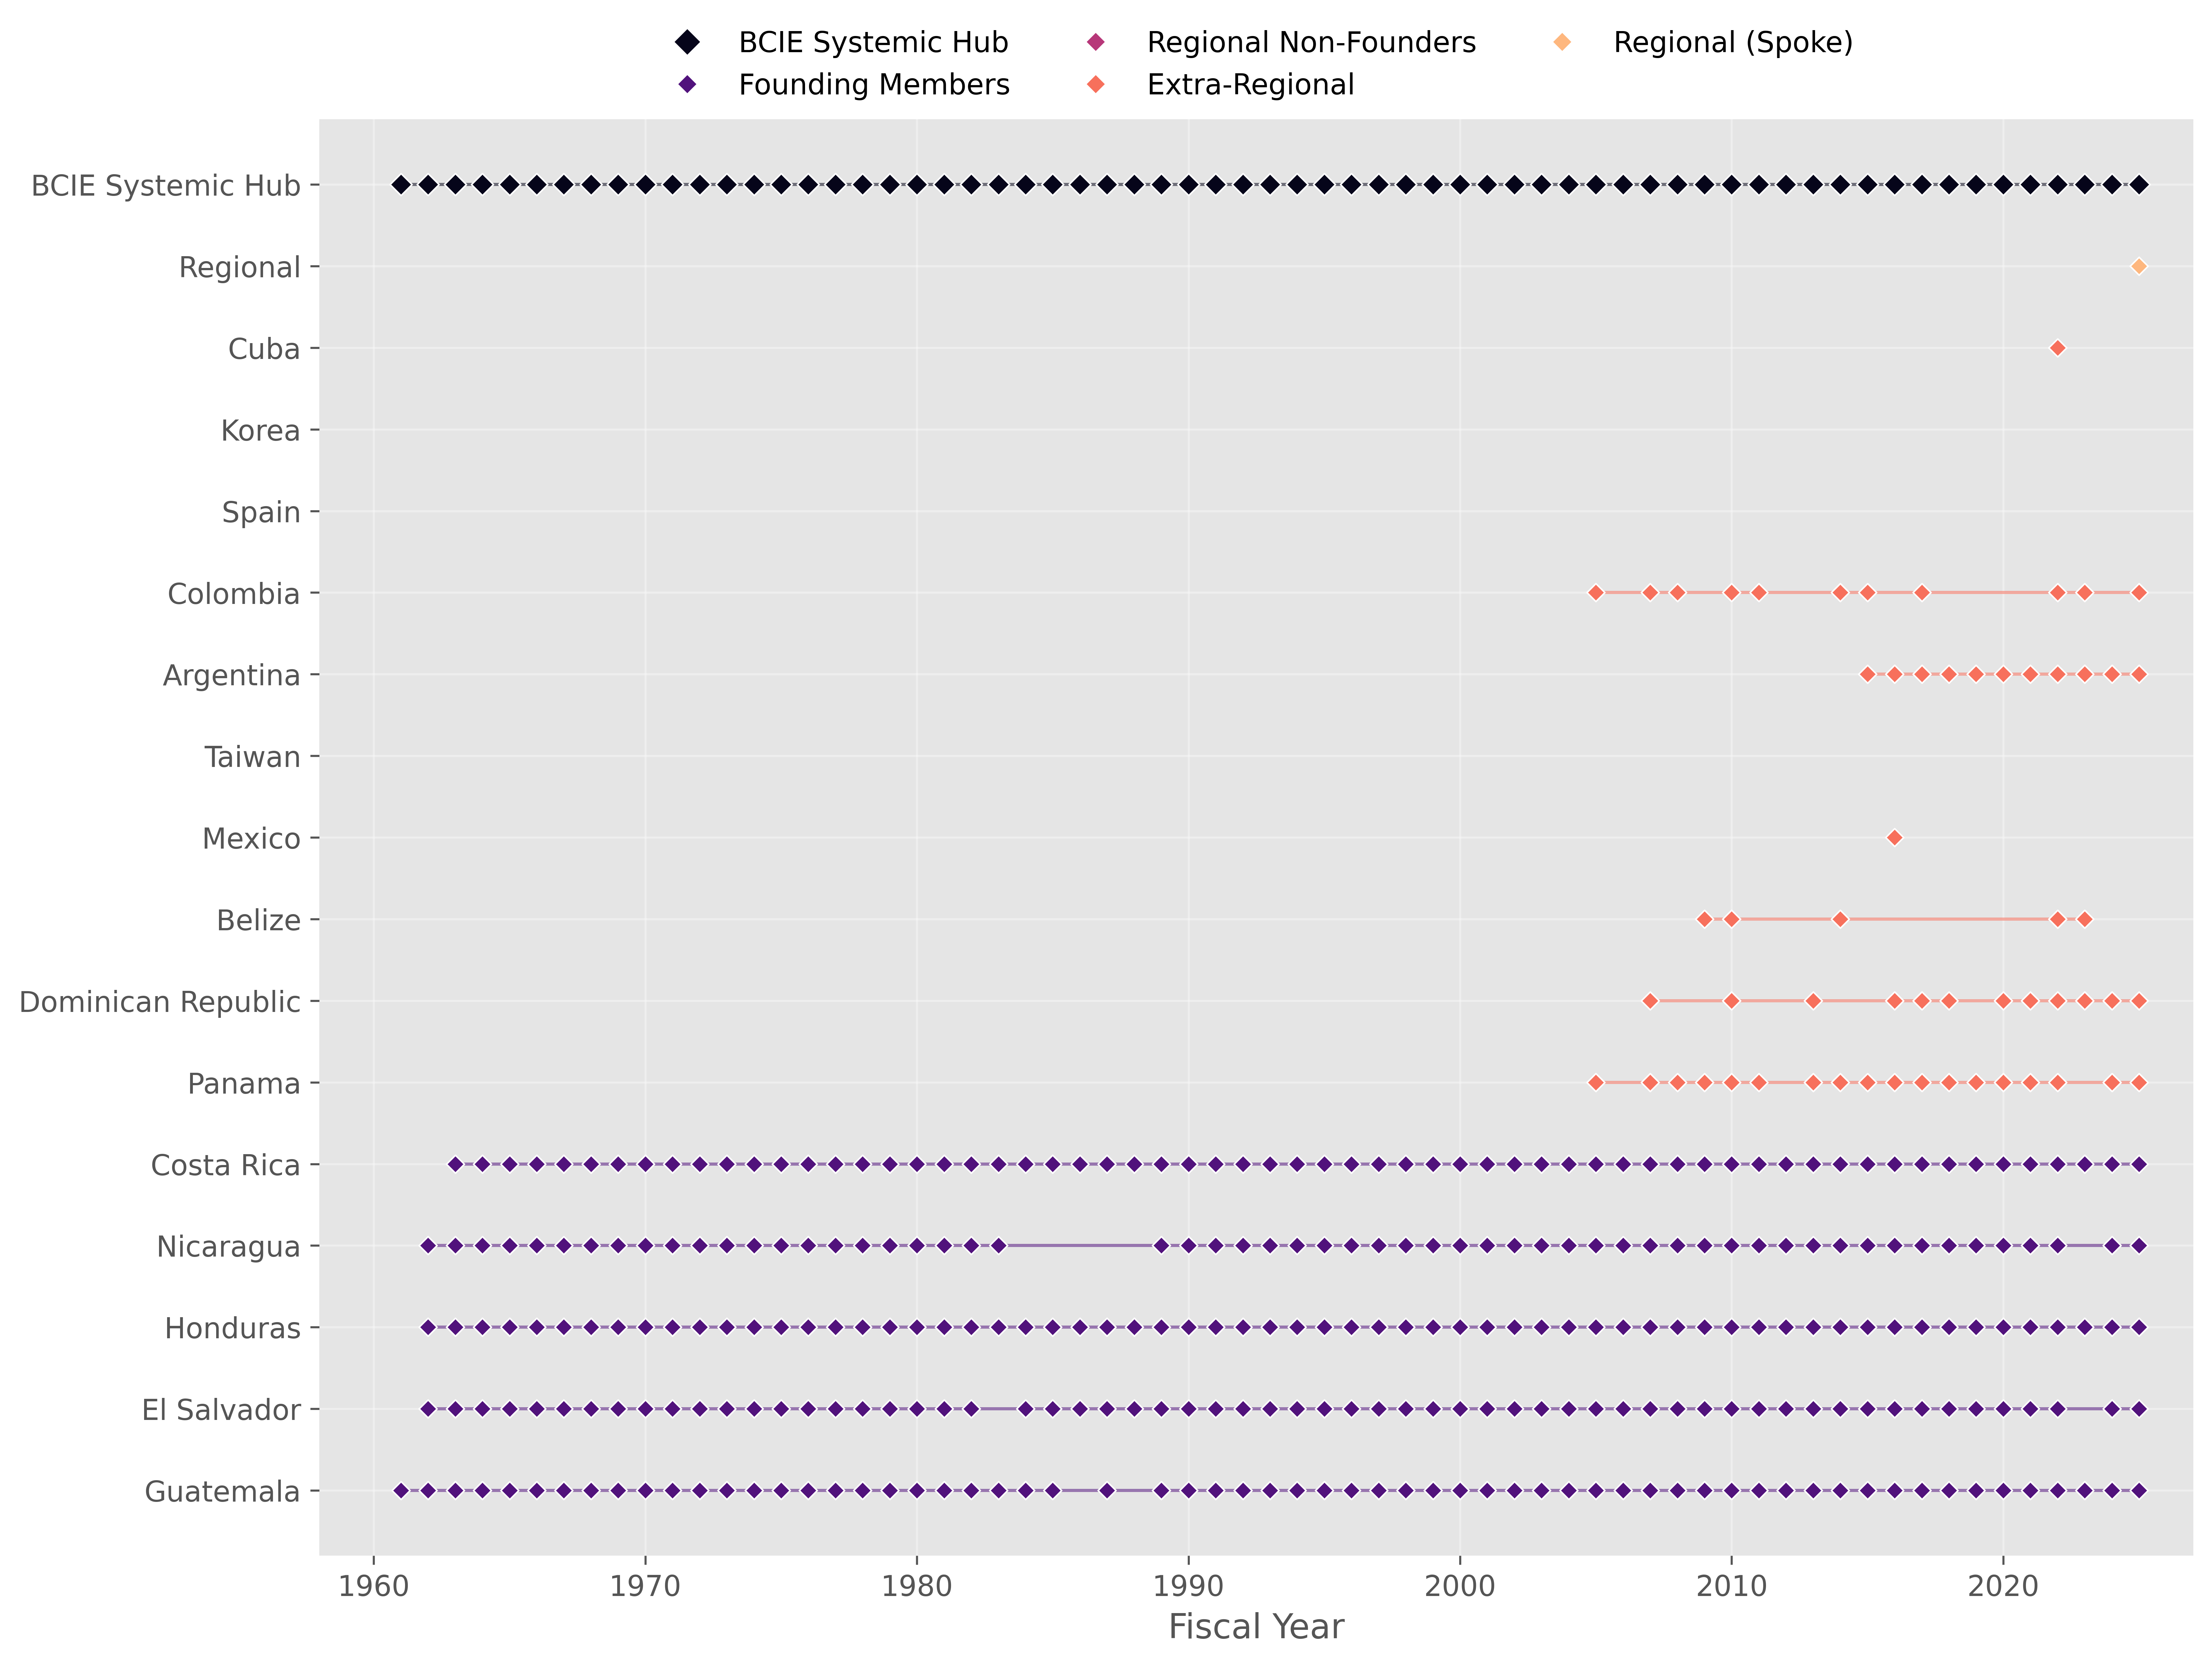
\includegraphics[width=0.9\columnwidth]{timeline_plot_16_1_EN.png}
\caption{Línea de Tiempo de Aprobaciones de Préstamos BCIE (Topología Jerárquica 16+1). El Hub Sistémico (arriba) agrega toda la actividad soberana y programática, proporcionando una señal continua para la estimación acoplada.}
\label{fig:timeline}
\end{figure}

La matriz de acoplamiento aprendida (Figura \ref{fig:heatmapP}) confirma que el Hub Sistémico actúa como el conductor dominante, mientras que acoplamientos fuertes específicos (por ejemplo, Argentina) destacan asociaciones estratégicas.

\begin{figure}[htbp]
\centering
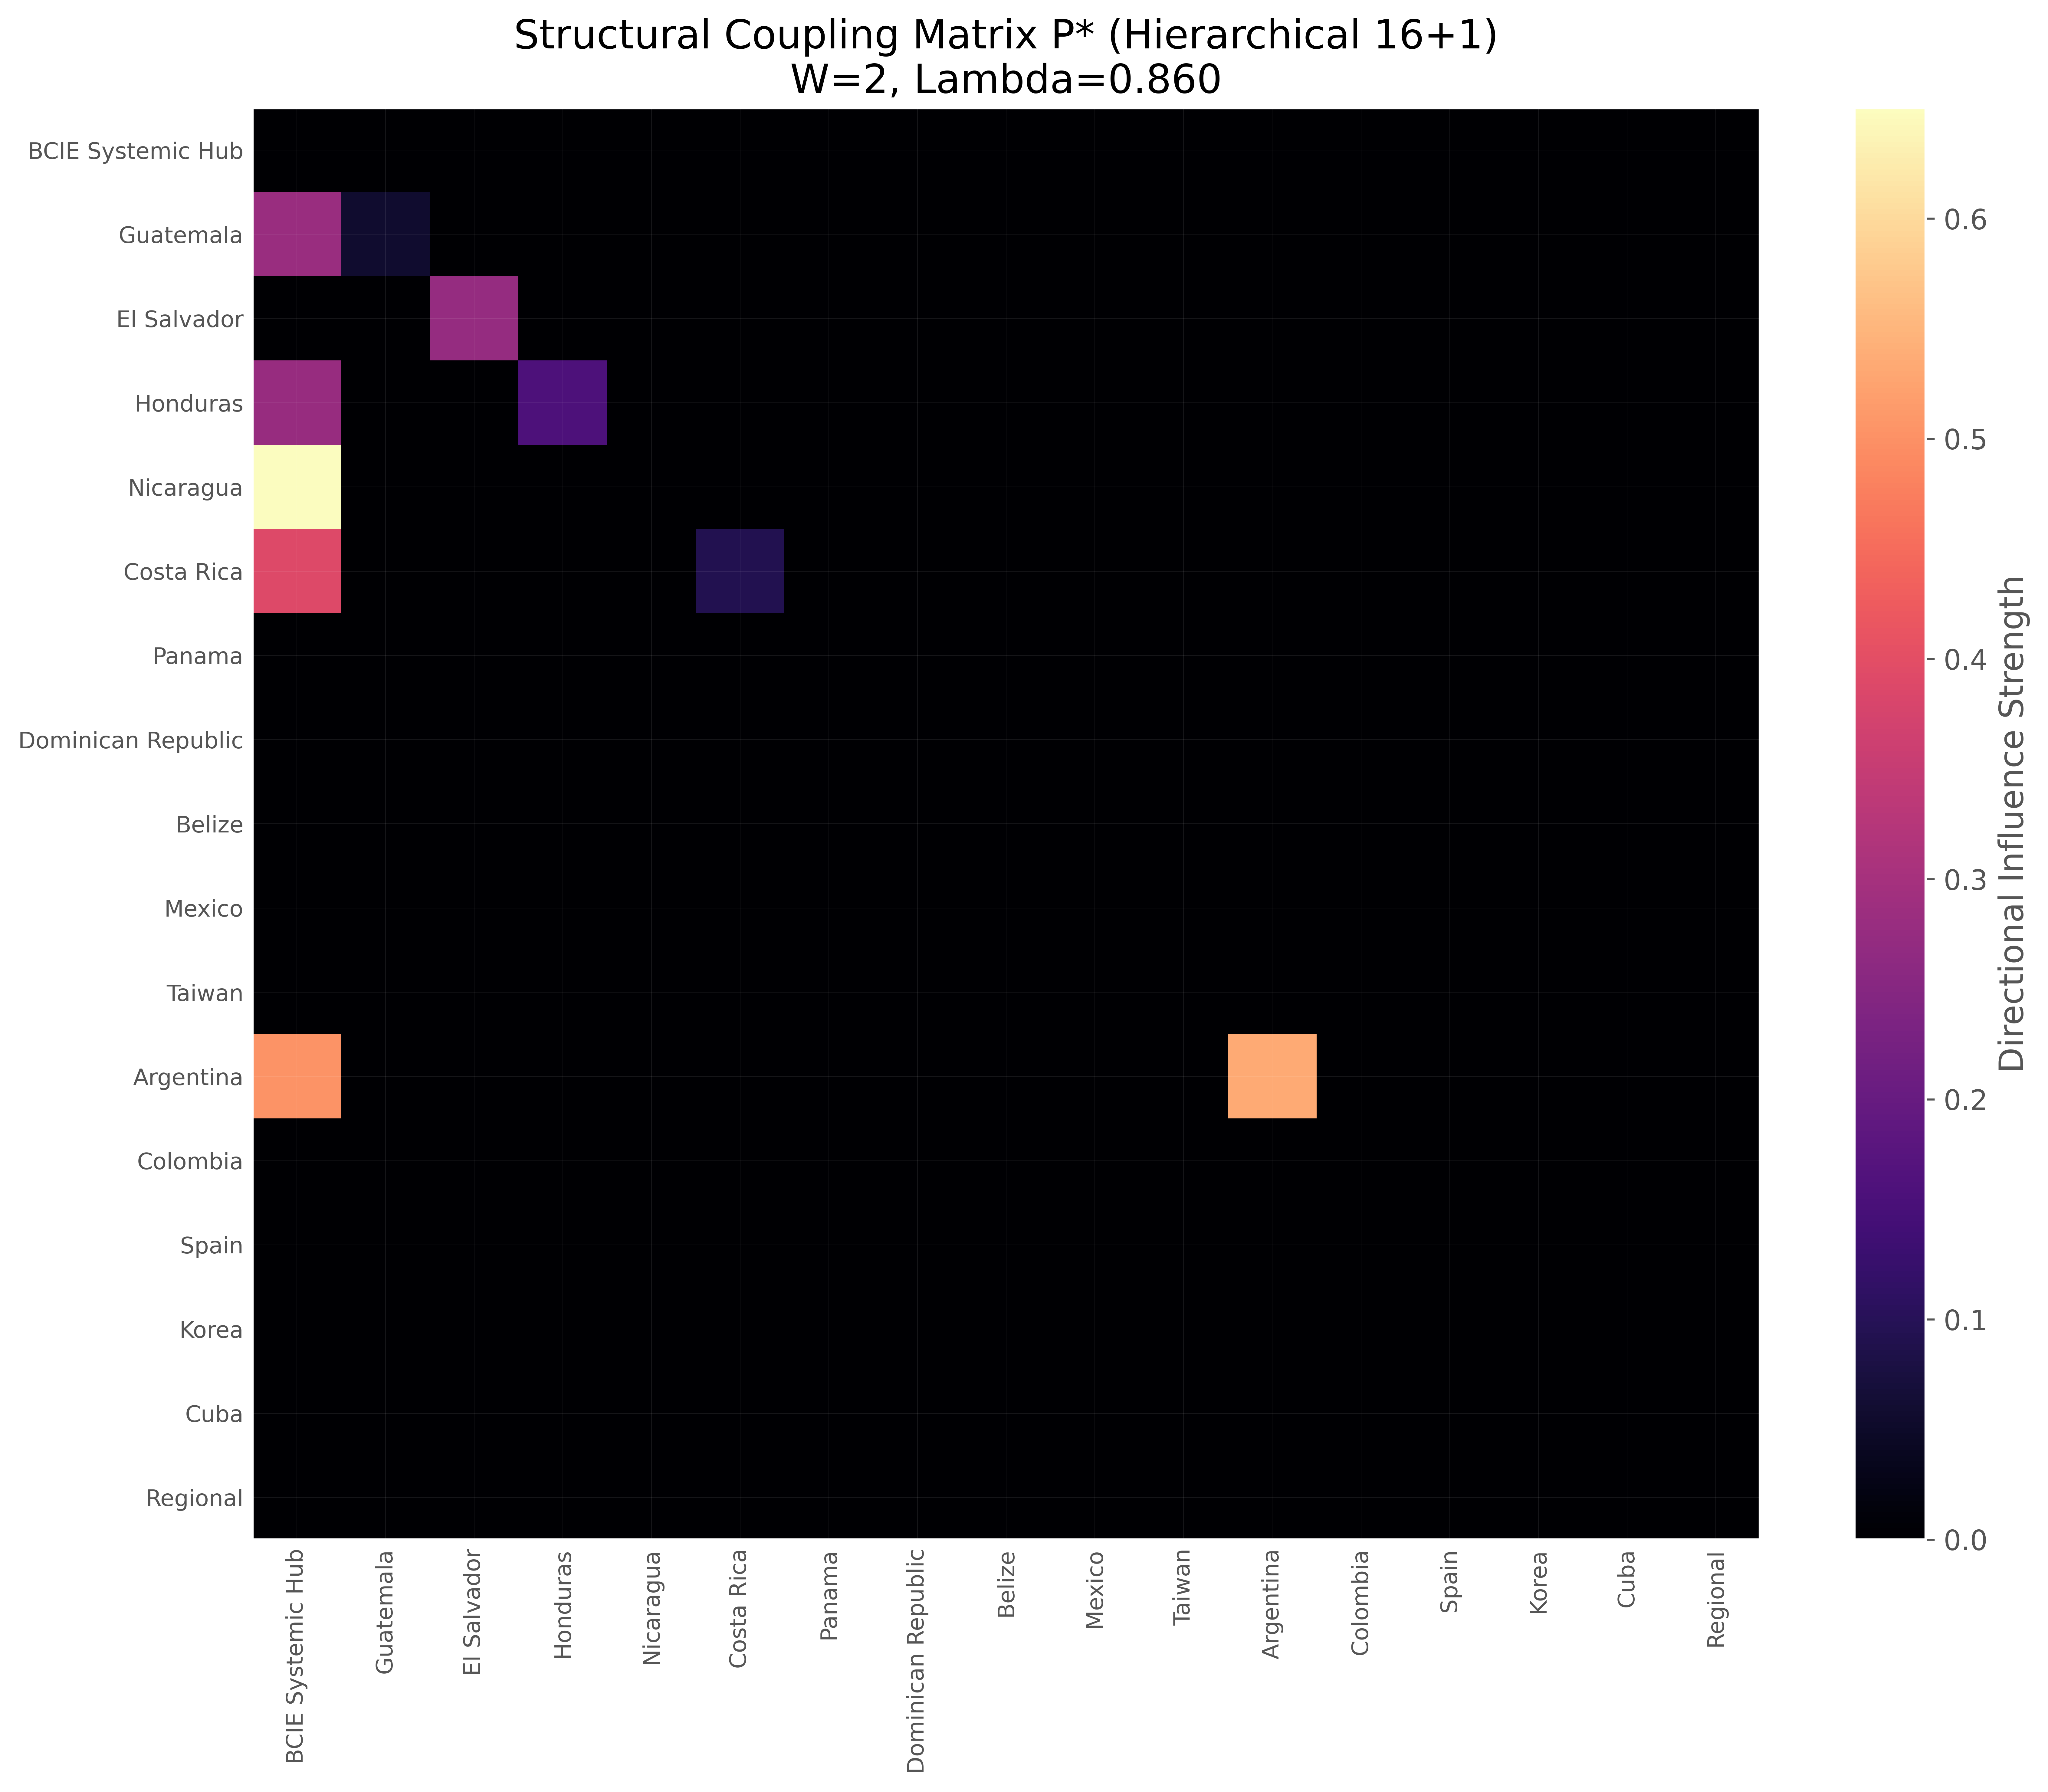
\includegraphics[width=0.9\columnwidth]{Final_P_Matrix_Hierarchical_Full.png}
\caption{Matriz de Acoplamiento Estructural Aprendida $\mat{P}^*$ (Topología Jerárquica 16+1). El Hub Sistémico (Fila 0) integra dinámicas, mientras que acoplamientos bilaterales específicos aparecen como puntos de interacción distintos.}
\label{fig:heatmapP}
\end{figure}

La descomposición de la dinámica del Hub Sistémico (Figura \ref{fig:alphaScale}) identifica claramente una ruptura estructural posterior a 2010, donde el volumen financiero y la frecuencia operativa divergieron, señalando un cambio hacia megaproyectos.

\begin{figure}[htbp]
\centering
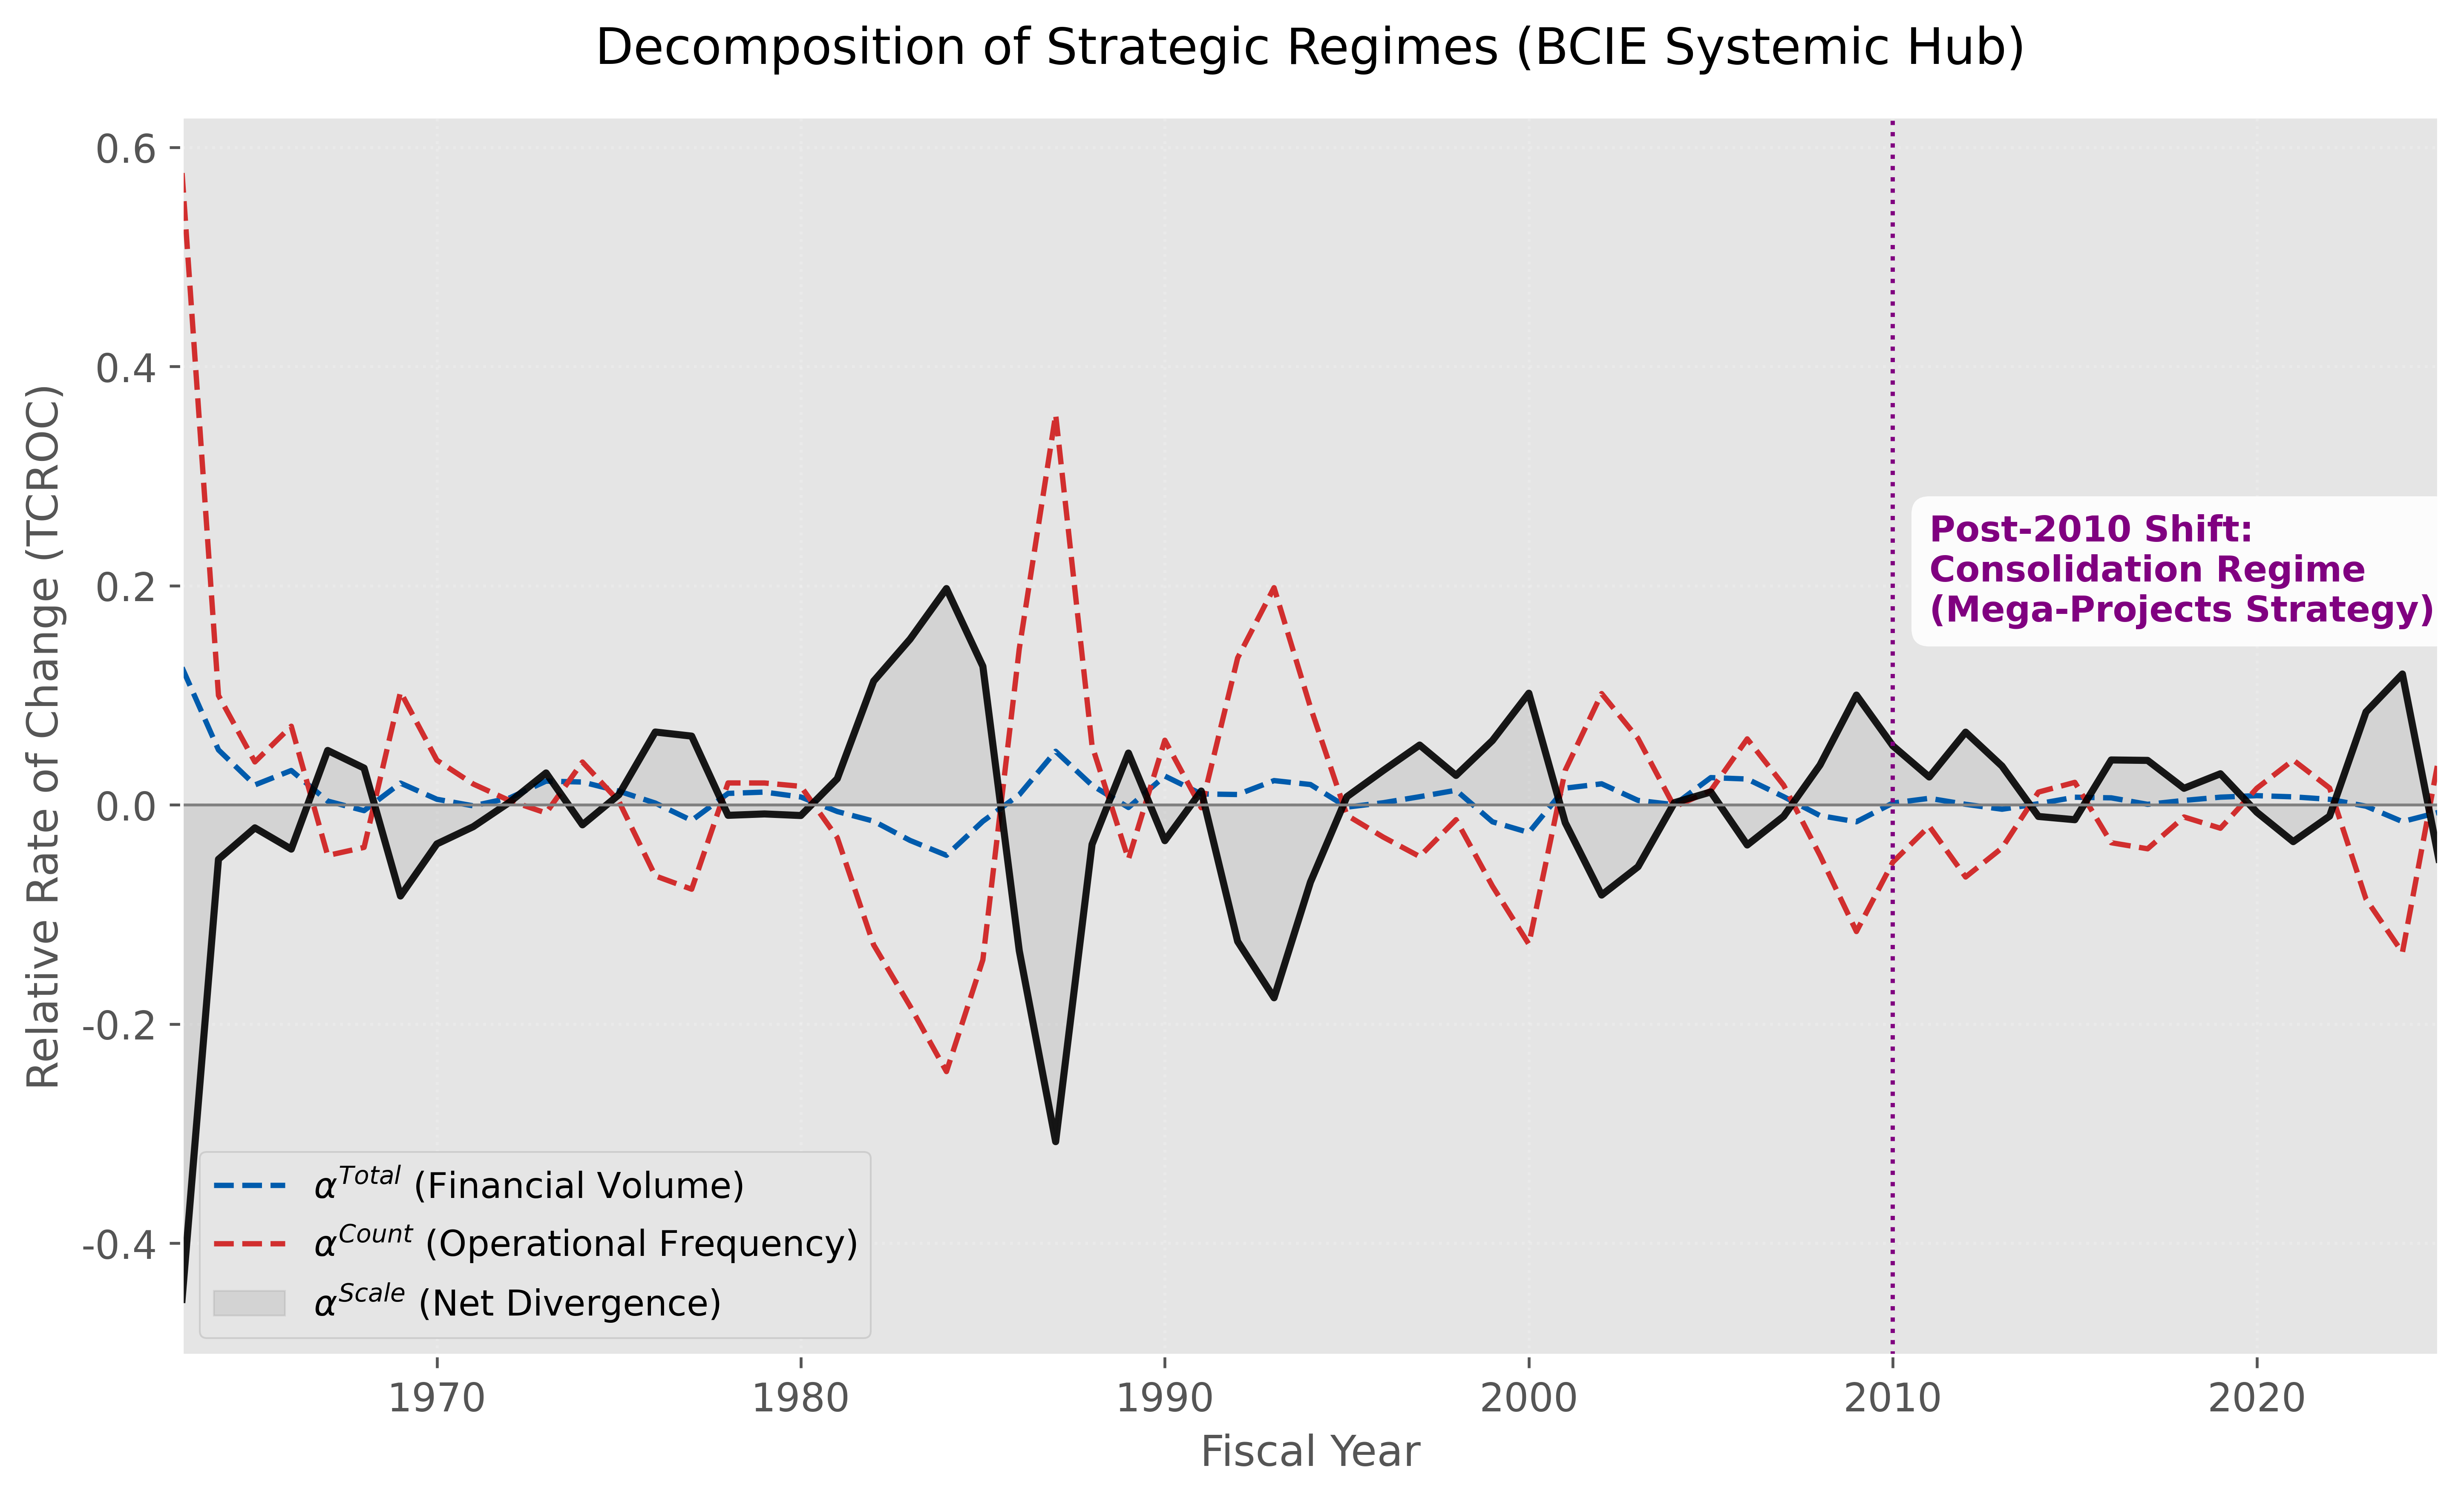
\includegraphics[width=0.9\columnwidth]{alpha_components_regional_v2.png}
\caption{Descomposición de Regímenes Estratégicos (Hub Sistémico BCIE). La divergencia entre Volumen Financiero (Azul Discontinuo) y Frecuencia Operativa (Rojo Discontinuo) revela el "Efecto Tijera" y el cambio de régimen de consolidación post-2010.}
\label{fig:alphaScale}
\end{figure}

\bibliographystyle{plain}
\bibliography{references}

\end{document}
